\documentclass{report}

% Pacotes para acentuação e formatação

\usepackage[utf8]{inputenc}
\usepackage[T1]{fontenc}
\usepackage[brazil]{babel}
\usepackage{setspace}    % Para espaçamento
\usepackage{lipsum}      % Texto de exemplo (remova se não precisar)
\usepackage{graphicx}


\begin{document}
	
	\begin{titlepage}
		
		\centering
		\vspace*{5cm} % Espaço do topo
		
		{\Huge\bfseries Estrutura de Dados I\par} % Título
		
		\vspace{0.5cm}
		{\Large 2025/2\par} % Ano
		
		\vfill
		{\large Nicolas Ramos Carreira\par} % Nome
		
		\vspace*{2cm}
	\end{titlepage}
	
	\tableofcontents
	\newpage
	
	\chapter{Intuito}
	
	O intuito deste documento é documentar o meu aprendizado da disciplina de estrutura de dados 1. Nesta disciplina começamos estudando sobre a linguagem C até entrar nas principais estruturas de dados. 
	
	\chapter{Fundamentos em C}
	\section{Sobre a linguagem C}
	A linguagem C é uma das linguagens de programação mais influentes e utilizadas da história da computação. Criada na década de 1970 por Dennis Ritchie nos laboratórios Bell, ela foi projetada para ser uma linguagem de propósito geral, eficiente e próxima do hardware, permitindo alto desempenho.
	
	C é considerada uma linguagem de médio nível, pois combina características de linguagens de baixo nível (como manipulação direta de memória) com recursos de alto nível (como funções e estruturas). Sua sintaxe influenciou muitas outras linguagens modernas, como C++, Java, Csharp e até mesmo Python em alguns aspectos.
	
	É amplamente usada em sistemas operacionais, softwares embarcados, drivers e aplicações que exigem alto desempenho. Além disso, aprender C é um ótimo ponto de partida para entender conceitos fundamentais de programação e arquitetura de computadores.
	\section{Estrutura de um programa em C}
		
	\begin{center}
		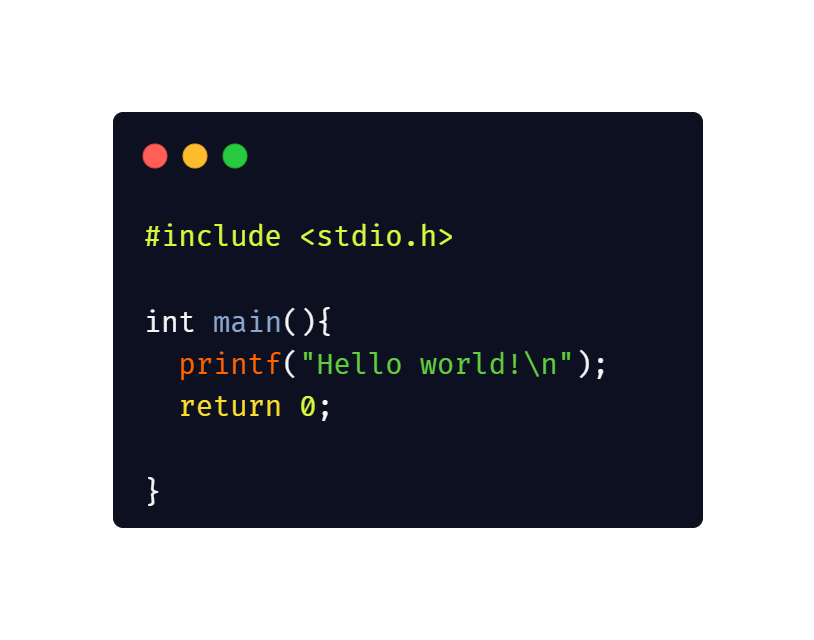
\includegraphics[width=6cm,height=5cm,keepaspectratio=false]{imagens/programac.png}
	\end{center}
	
	A imagem acima mostra um programinha extremamente simples em C, um Hello, world. Para iniciar um programa em C, nós sempre começamos declarando a biblioteca principal, que é a stdio.h (poderíamos ter outras bibliotecas inclusive, mas essa é a principal e DEVE estar lá). 
	
	Depois disso, nós declaramos o local do programa principal, onde fazemos o programa em si. 
	
	Um detalhe é que ao final de cada coisa SEMPRE temos que ter o ponto e vírgula (;), pois se não o nosso programa não compila.
	
	\section{Aspectos da linguagem C}
	\subsection{Variaveis}
	\subsubsection{O que são e pra que são usadas}
	Varivel, em linguagens de programação, é basicamente uma posição alocada da memória para guardar uma informação. Variaveis podem ser modificadas pelo programa e devem ser definidas antes de ser utilizadas
	\subsubsection{Declaração de variaveis em C}
    Para definir variaveis em C, nós precisamos passar o tipo de dado e nome da variavel, no formato: <tipo de dado> nome-da-variavel. O tipo de dado deve ser aqueles que são aceitos pela linguagem (inteiro, decimais, caracteres, booleanos..), mas como falaremos sobre tipos de dados mais pra frente, não entraremos em detalhes agora. O nome da variavel é algo bem importante a se considerar, pois existem algumas regras e boas práticas importantes quanto a isso:
    \begin{itemize}
    	\item Nomes de variaveis devem iniciar com letras ou underscore 
    	\item Os caracteres da variavel devem ser letras, numeros ou underscore (não utilizar acentos ou simbolos)
    	\item Não utilizar espaço em nomes de variaveis
    	\item Palavras chaves (palavras que são reservadas pela linguagem para fazer determinadas coisas) não podem ser usadas como nomes 
    	\item Letras maiusculas e minusculas são consideradas diferentes
    \end{itemize}
    
    Só para deixar totalmente claro, as palavras chaves que a linguagem C usa são:
    
    \begin{figure}[ht]
    	\centering
    	% ajusta a largura da imagem para ser quadrada (ex: 5cm x 5cm)
    	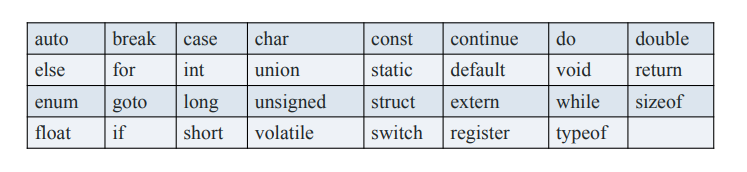
\includegraphics[width=9cm,height=2cm,keepaspectratio=false]{imagens/reservadas.png}
  
    \end{figure}
    
    \subsubsection{Atribuição de valores em variaveis}
    
    Tendo o formato <tipo de dado> nome-da-variavel, podemos atribuir valores a elas (ou seja, armazenar valores dentro da memória). Para isso, basta fazer:
    
    \begin{LARGE}
    	\begin{center}
    		<tipo de dados> nome-variavel = valor
    	\end{center}
    \end{LARGE}
    
	\subsection{Tipos de dados}
	Como falamos anteriormente na parte de variaveis, quando vamos defini-las, nós temos que declarar o tipo de dado da variavel. O tipo de dado define os valores que aquela variavel pode assumir e as operações que podem ser realizadas com ela.
	Os tipos de dados principais são: char, int, float e double
	\subsubsection{Char}
	Um byte que armazena
	\subsubsection{Int}
	Um inteiro cujo o tamanho do numero que pode ser alcançado depende do processador (tipicamente 16 ou 32 bits)
	\subsubsection{Float}
	Basicamente numeros decimais com precisão simples (em C a parte decimal usa ponto e não vírgula)
	\subsubsection{Double}
	Também números decimais, mas com precisão dupla. É usados para numeros muito pequenos (cientificos por exemplos) ou muito grandes
	\subsubsection{Outros tipos}
	Na imagem abaixo, você poderá ver alguns outros que são utilizados:
 	\begin{center}
		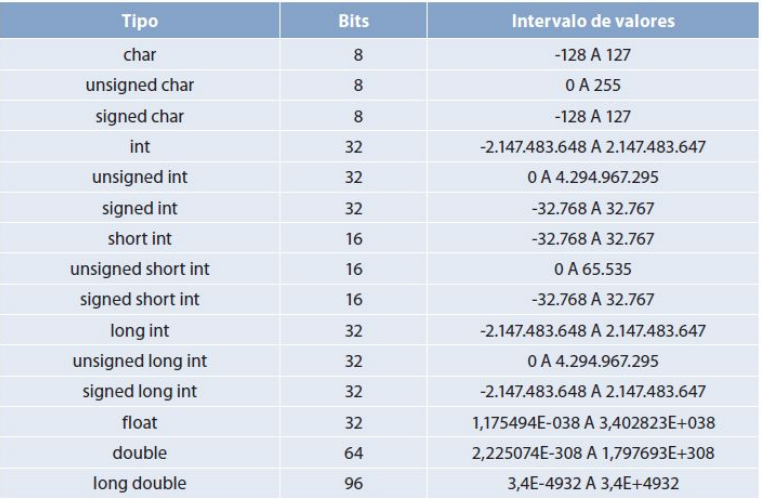
\includegraphics[width=8cm,height=7cm,keepaspectratio=false]{imagens/tipos.png}
	
	\end{center}
	
	\subsection{Input e output}
	Input e output é basicamente a entrada e a saída de dados. As vezes, podemos querer receber do usuário alguns valores, para fazer alguma coisa com eles e depois entregá-los com modificações. É basicamente isso. Um detalhe é que para o output, não necessariamente nós precisamos ter recebido algo.
	\subsubsection{Especificadores de formato}
	\subsubsection{Saída com printf()}
	Vamos começar com a saída de dados. Para exibir algo na tela. Fazemos:
	\begin{figure}[ht]
		\centering
		% ajusta a largura da imagem para ser quadrada (ex: 5cm x 5cm)
		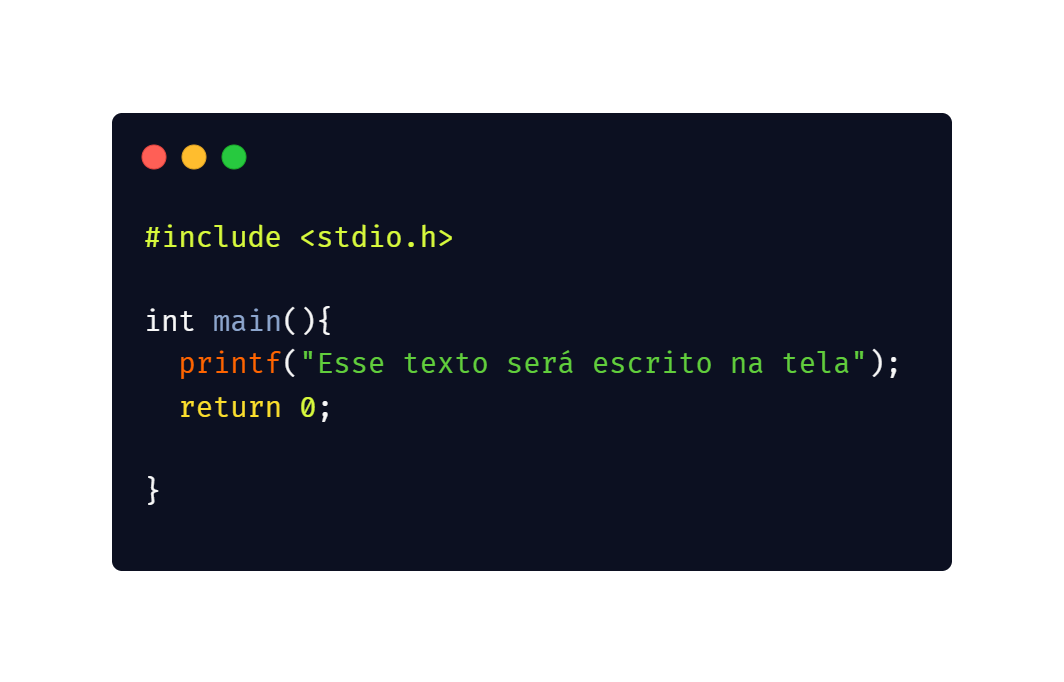
\includegraphics[width=6cm,height=3cm,keepaspectratio=false]{imagens/print.png}
		
	\end{figure}
	
	Ao fazer isso, em nosso terminal será exibido o texto que digitamos dentro do printf ("Esse texto será escrito na tela). Veja
	
	\subsubsection{Uso do escape no printf()}
	Um detalhe é que algo que podemos utiliza no printf é caracter de escape . Esse caracter é utilizado sempre ao final do que que queremos escrever na saída e ele serve para quebrar a linha após a saída. Veja:
	
	\begin{figure}[ht]
		\centering
		% ajusta a largura da imagem para ser quadrada (ex: 5cm x 5cm)
		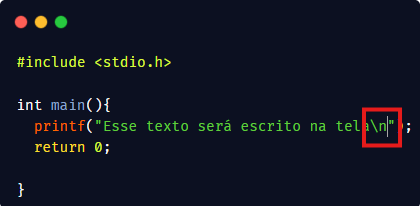
\includegraphics[width=6cm,height=3cm,keepaspectratio=false]{imagens/escape.png}
		
	\end{figure}
	
	
	Se fizermos vários printf, por exemplo, e não usarmos o caracter de escape em nenhum deles, o que escrevemos nos prints, ficará tudo junto. Veja
	\subsubsection{Entrada com scanf()}
	\subsection{Contantes}
	Assim como variaveis, constantes também armazenam um valor na memória do computador. A principal diferença para as variaveis é que esse valor não será alterado. Outra coisa é que para as constantes é obrigatoria a atribuição de valor, diferente das variaveis que podemos simplesmente declará-las sem dar um valor
	\subsubsection{Declaração de constantes}
	Para declarar uma constante existem duas formas. Na primeira, devemos  utilizar define nome-costante <valor> no começo do programa. Veja:
	
	Outra forma é fazer const <tipo> nome = valor
	\subsection{Operadores}
	Os operadores são usados para desenvolver diferentes tipos de operações. Com eles podemos fazer operações matematicas, comparativas, logicas e etc. Veremos acerca de cada um dos operadores a seguir
	\subsubsection{Operadores aritméticos}
	\subsubsection{Operadores relacionais}
	\subsubsection{Operadores lógicos}
	\subsection{Coerção de tipos}
	\subsection{Condicionais}
	\subsubsection{If-else}
	\subsubsection{Swicth-case}
	\subsection{Loops}
	\subsection{Arrays}
	\subsection{Struct - Criação de tipos}
	
	\chapter{Falando sobre ponteiros}
	

\end{document}

